\documentclass[12pt,a4paper,english,twoside]{book}
\usepackage[german,english]{babel}
\usepackage[T1]{fontenc} 
\usepackage[latin1]{inputenc}
\usepackage{amsfonts}
\usepackage{amsmath}
\usepackage{latexsym}
\usepackage{amssymb}
\usepackage{pifont}
\usepackage{epsfig}
\usepackage{moreverb}
\usepackage{rotating}
\usepackage{enumerate}
\usepackage{graphics, graphicx,wrapfig}
\usepackage{fancybox}
\usepackage{picinpar,varioref,floatflt}
\usepackage{ae}
\usepackage{longtable}
\usepackage{textcomp}
\usepackage{float}
\usepackage{url}
\usepackage{unizhdt}
\usepackage{setspace}
\usepackage{refstyle}
\usepackage{listings}
\newcommand{\cmark}{\ding{51}}%
\newcommand{\xmark}{\ding{55}}%
\graphicspath{ {./graphics/} }
\newcommand{\code}[1]{\texttt{#1}}
\lstdefinestyle{CEE}{language=C, frame=l,  numbers=left,  numbersep=1em,  xleftmargin=2em} 
\lstdefinestyle{ASS}{language=[x86masm]Assembler, frame=l,  numbers=left,  numbersep=1em,  xleftmargin=2em} 
\lstdefinestyle{SH}{language=sh, frame=l, numbers=left} 
\lstdefinestyle{LD}{language=sh, frame=l} 


%%%%%%%%%%%%%%%%%%%%%%%%%%%%%%%%%%%%%%%%%%%%%%%%%%

% Define the language of the diploma thesis
\selectlanguage{english}
%\selectlanguage{german}

\pagestyle{headings}

\begin{document}

%%%%%%%%%%%%%%%%%%%%%%%%%%%%%%%%%%%%%%%%%%%%%%%%%%

% Define the author printed on the cover page
\author{Filip Dombos}
% Define the city and country of the author
\authorcity{Baden, Switzerland}
% Define the student ID (Matrikelnummer)
\studentid{14-939-664}
% Define the title with optional subtitle
\title{Linux on Tiny Microcontrollers}
% Define the supervisors
\supervisors{Eryk Schiller}
% Define the submission date
\submissiondate{July 27, 2022}

%%%%%%%%%%%%%%%%%%%%%%%%%%%%%%%%%%%%%%%%%%%%%%%%%%

% Make the title page
\maketitle

% Make the imprint on the back of the cover page
\makeimprint

\pagenumbering{roman}

\onehalfspacing
% \doublespacing

% Include the files of the diploma thesis
\chapter*{Abstract}
\addcontentsline{toc}{chapter}{Abstract}

\selectlanguage{german}

Das ist die Kurzfassung... \cite{8101926}

HELLO CITERS\cite{website1}


\selectlanguage{english}

This is the summary for the english language

\chapter*{Acknowledgments}
\addcontentsline{toc}{chapter}{Acknowledgments}
\selectlanguage{english}

First and foremost, I would like to thank my research supervisor, Dr. Eryk Schiller, without whom this thesis would not have been possible. I would like to thank, Dr. Eryk Schiller for his guidance, patience, for every meeting we held, and his high-level insights on the topic at hand. Furthermore, I want to extend my gratitude to Prof. Dr. Brukhard Stiller for providing me with the opportunity to write my bachelors thesis at the Communication Systems Group (CSG) in the University of Zurich.

Thanks also goes to STM Technical Marketing Manager Marco Sanfilippo and STM as a company, for providing us with feedback, consultation, and with two STM32L4 development boards, on which we performed some tests.


\tableofcontents

\pagenumbering{arabic}
\chapter{Introduction}

\section{Motivation}

In the previous two decades, the development and use of sensing- and connectivity-enabling electronic gadgets has steadily increased, in some areas substituting conventional physical devices~\cite{schiller}. With a central focus on interconnectedness, the appropriately named, Internet of-Things (IoT) refers to the billions physical gadgets connected to the internet of throughout the world, all gathering, and more importantly, sharing massive amounts of data. IoT has become an integral part of the lives of billions of people worldwide, not only due to the sheer number of connected devices and potential use cases~\cite{iot-size} but also due to the diversity and variety of IoT solutions~\cite{banafa2016iot}. Many people believe that IoT is the essential development of the twenty-first century, because it affects almost every industry, from healthcare to transportation. However, as the world around us becomes increasingly linked, protecting these resource-constrained devices has become critical.

Linux runs on some microcontrollers, such as the Raspberry Pi (RPI) family. For example, RPI 3B is a small computer equipped with computing essentials, e.g., the Advanced RISC Machines (ARM) Cortex central processing unit (CPU), Random Access Memory (RAM), but not necessarily of the latest generation, having minor energy requirements. As an example, instead of a hard drive, an RPI is equipped with a flash memory card, on which an Operating System (OS) may be installed. It also offers Universal Serial Bus (USB) connectors, a video output, and a Wireless Fidelity (Wi-Fi) adapter. As RPI is a small computer, a regular general-purpose OS such as Linux-based Ubuntu for the ARM architecture can also be supported. However, Raspberry Pi OS, previously known as Raspbian, is a typical distribution of choice for the Raspberry Pi device family. Linux is an excellent success on Raspberry Pi as it simplifies the development of microcontroller applications, as a regular operation can be used with which users are already familiar. Currently, a new generation of microcontrollers is being introduced into the market. For example, the ESP32 device family is based on the dual-core Reduced Instruction Set Computer (RISC)-based Tensilica LX6 processor with a maximum frequency of 240 MHz, 8 MB PSRAM, and 4 MB flash seems to be a great choice to run Linux on those devices as well. Linux was first developed for the Complex Instruction Set Computer (CISC)-based Intel 386 (i386) architecture in 1991. Back then, the typical CPU clock speed of the i386 system was between 12 MHz to 40 MHz, while the typical computer was equipped with several megabytes of RAM (e.g., 4 MB). As ESP32 already exceeds the specification of early i386 systems, it seems to be that porting Linux for those devices shall be possible. 8 megabyte (MB) pseudo-static RAM (PSRAM) on ESP32-WROVER-IE shall be satisfactory to run the kernel, uclibc, and essential binaries. 

The cheapest development board for ESP32-WROVER-IE costs around 10 CHF. However, when one does not need a development board, an ESP32-WROVER-IE costs 3 CHF. Regular RPI 0 devices, which already contain an ARM Cortex CPU, cost 22-24 CHF, while an RPI 3 costs around 38 CHF. The cost reduction from RPI 3 to Linux-capable ARM-based RPI 0 is already 42\%, and the further cost reduction from RPI (Zero development board) to ESP32-WROVERIE would be another 54\%. Running Linux on regular ESP32-WROVER-IE (i.e., not with a development board) would mean a cost reduction of 92\% in comparison to an RPI 3 device. This is a massive incentive to port a Linux-based distribution towards the new family of devices. The migration of Linux on ESP32 should be possible as there is already a Linux kernel project supporting the kernel execution on the Tensilica LX6 processor family.

RISC-V is another open standard instruction set architecture (ISA) that was first released in 2010 and is based on RISC (Reduced Instruction Set Computer) principles. A layered security method that employs a Trusted Execution Environment (TEE) provided in the RISC-V architecture is a gamechanger in the IoT industry. Unlike most other ISA designs, RISC-V is available under open-source that does not require license fees. RISC-V hardware is available from several companies. Opensource operating systems with RISC-V support are available, and many major software toolchains support the instruction set. Furthermore, there is a Linux kernel available for the RISC-V processor family. As an example, the Espressif ESP32-C3 is a single-core, 32-bit, RISC-V-based MCU with 400KB of SRAM and a 160 MHz clock speed. It includes 2.4 GHz Wi-Fi and Bluetooth 5 (LE) with built-in long-range capability.


\section{Description of Work}

The focus of this thesis is to lay a foundation for porting the open source software (OSS) Linux kernel to tiny microcontrollers and to provide a Linux distribution for future studies, which people can use, and upon which they can build. As the first step, a market analysis must be performed to find suitable MCU boards that can support Linux. Then correct toolchains and libraries need to be found to successfully compile Linux targeted at these tiny edge devices. Having compiled the Linux source code, correctness needs to be verified using QEMU, and as the last step flashing the code onto the chosen device.

\section{Thesis Outline}
This thesis is segmented into seven chapters. Related Work in Section 2 provides a description of IoT architectures, security, operating systems, and the lack of standardization. In Section 3 we establish what devices this thesis considers, perform a market analysis, and introduce various tools and projects that were used within the thesis. Section 4 proposes a way towards standardization, and outlines the goal. In Section 5 we set up an environment with the tools discussed in Section 3, and sample code, that helps us to evaluate, is introduced and explained. Finally, in Section 6 we evaluate the tools and projects, with a conclusion following in Section 7.


\chapter{Related Work}

\section{The Internet-of-Things}

There was already a market for microcontrollers at the time Intel introduced the 4004 as the first single-chip microprocessor. By the end of 1971, Texas Instruments began marketing the TMS1802, a modern calculator designed for use in cash registers, watches, and measurement devices. But the first MCU's that gained widespread use were Intel's next generation 8-bit controllers, such as the Intel 8048 and Intel 8051 operating on the MCS-51 instruction set architecture (ISA), most notably used in Desktop peripherals such as the keyboards. While these MCU's build the foundation of IoT, the edge hardware, the first primitive IoT device, a toaster that can be turned on and off remotely, was introduced in 1990~\cite{7786805}.

The phrase "Internet of Things", was initially coined by Kevin Ashton in 1999. Ashton made the initial proposal for the Internet of Things (IoT), which he defined as a network of radio-frequency identification (RFID)-enabled, interoperable, linked items. IoT can include billions of intelligent, communicative "things", enabling connections between people and these things at any time, anywhere, with anything, and with anybody, preferably via any path/network and any service. Thus envisioning a system in which omnipresent and ubiquitous devices will link the Internet to every physical object~\cite{shin2014socio, wang2015introduction}.

% transition isn't too smooth...
The quantity and diversity of IoT devices and solutions have multiplied due to the markets quick development. According to IoT reports, there were between 6.1 billion and 8.4 billion IoT devices in use in 2017, in 2020 growing to 20.4 billion, and by 2025 it is anticipated that there will be 75 billion IoT devices~\cite{iot-size1, iot-size2}. Although others report fewer devices \cite{iot-size3}, the same upwards trend is captured. 
% weird sentence
This discrepancy is indicative of the diverse manufacturers, countless forms, and the enormous amount of devices, that make it challenging to identify a precise quantity. 
%
Despite the lack of definitive numbers, it clearly shows that IoT has become more relevant and omnipresent, with growth that isn't showing any signs of slowing. 

% about the uses of IoT
With Governments heavily investing into initiatives such as the UK's Future Internet Initiatives, the European Research Cluster on IoT, the National IoT Plan of China's Ministry of Industry and Information Technology, the Italian National Project of Netergit, and Japan's u-Strategy~\cite{shin2014socio}. Uses of IoT are numerous, including medical, industrial, and consumer. Examples include ............. ............ .............. and automatic irrigation systems for farms \cite{tarange2015web}.



\section{IoT Architecture}
But IoT does not only encompasss the tiny edge devices. It includes sensing, computing, networking, and cloud. Yet there is no concensus regarding IoT architecture, a multitude of models have been proposed, the most basic of which being the three-layer architecture~\cite{sethi2017internet}. 

\begin{enumerate}
\item The physical layer, which contains sensors for perceiving and gathering environmental data, is the perception layer. It detects certain physical factors or other intelligent things in the surrounding area.

\item The network layer is in charge of establishing connections with other intelligent objects, network components, and servers. Its capabilities are also employed for processing and transferring sensor data. Notably IPv6........

\item The application layer delivers application-specific services to the user is the responsibility. It describes a variety of uses for the IoT, including smart homes, smart cities, and smart health.
\end{enumerate}

[SHOW FIGGURE HERE]



\section{The lack of standardization}
% needs a reference.
[I had a really good quote here, but I can't find it anymore... something about the consequence of rapid development, and the need to standardize]
As a result of the rapid development of IoT, the industry has concentrated on creating and delivering the appropriate kinds of hardware. In the current model, the majority of IoT solution providers have been building all components of the stack, from the hardware devices to the relevant cloud services, or as they call it "IoT solutions"~\cite{banafa2016iot}.

As interoperability is ensured by standardization, it improves the effective integration and information exchange between distributed systems. But manufacturers are using own standards which inevitably has the effect that devices can not talk to each other. \cite{al2016iot} conclude that the lack of standardization negatively impacts the IoT industry.

The requirement for a standard model to carry out typical IoT backend functions, such as processing, storing, and firmware upgrades, is growing in importance as the industry develops. Different IoT solutions are expected to cooperate with shared backend services in this new architecture, which will provide levels of interoperability, portability, and management that are almost unattainable with the current generation of IoT systems~\cite{banafa2016iot}.

"The Internet of Things Might Never Speak a Common Language"~\cite{newman2016internet}.




\section{IoT Security Issues}

The term IT-Security was defined as follows. Information integrity, availability and confidentiality~\cite{voydock1983security}. In a paper by Schiller et al. \cite{schiller} security is defined as message confindentiality. This is exclusively the case if only the sender and receiver are aware of the existence of the message and only they can verify its validity.

The security strategies and procedures that have been suggested are mostly based on traditional network security procedures. However, given the variety of the devices and protocols including the quantity of nodes in the network, implementing security methods in an IoT system is more difficult than with a typical network~\cite{hassan2019current}.

\section{Operating Systems on IoT} \label{iotos}

\cmark

Linux is a monolithic kernel..... elaborate on this.
\cite{milinkovic2015choosing} have analysed different OS's for IoT edge devices. By compiling a list of  
\cite{milinkovic2015choosing} goes as far as stating that "Linux will never run on these chips", by chips refering to ARM Cortex-M series.
\cite{sabri2017comparison}


\begin{sidewaystable}[h!]
	\centering
	
	\begin{tabular}{c|c|c|c|c|c|c|c|c}
	OS & Min RAM & Min ROM & C Support & C++ Support & Multi-Threading & MCU w/o MMU & Modularity & Realtime\\
	\hline
	\hline
	Linux & $\thicksim$1MB & $\thicksim$1MB  & \cmark & \cmark & \cmark & \xmark & $\circ$ & $\circ$ \\
	Contiki & <2kB & <30kB  & $\circ$ & \xmark & $\circ$ & \cmark & $\circ$ & $\circ$ \\
	Tiny OS & <1kB & <4kB  & \xmark & \xmark & $\circ$ & \cmark & \xmark & \xmark \\
	RIOT & $\thicksim$1.5kB & $\thicksim$5kB  & \cmark & \cmark & \cmark & \cmark & \cmark & \cmark \\
	\end{tabular}
	\caption{Key characteristics of TinyOS, Contiki, RIOT, and Linux}
	\label{tab:my_label}
\end{sidewaystable}




\section{Summary}

With huge potential and growth to satisfy the rapid demand
\chapter{Overview of Hardware \& Technologies}

Due to the explorative nature and the width of this thesis, we have to introduce a variety of different IoT ISA's, System-on-a-Chip manufactureres and their relevant products, open source projects with the aim to aid in the process of embedding, toolchains, and technologies. This chapter serves as an overview of the various devices and tools that were discovered, and may help further research which aim to achieve similar goals.

\section{Micro Computing}
Von Neumann's Architecture states that a modern computer requires a couple of core components to be able to run~\cite{arikpo2007neumann}. Figure \ref{fig:vonNeumanng} shows a visual representation.
\begin{itemize}
\item A \textbf{Processor Unit}, or a \textbf{core processing unit (CPU)} can further be divided into two subcomponents, the Controll Unit (CU) and the Arithmetic Logic Unit (ALU). This component performs operations and instructions on the data stored in the main memory unit and on the I/O devices.
\item The \textbf{Main Memory Unit}, or simply memory, stores data and the operations that need to be performed on this data.
\item The \textbf{Input/Output (I/O) Devices}, can be anything that allows us to interact with the computer, such as a mouse or keyboard, or simply just an LED light that gets turned on.
\end{itemize}

\begin{figure}
\centering
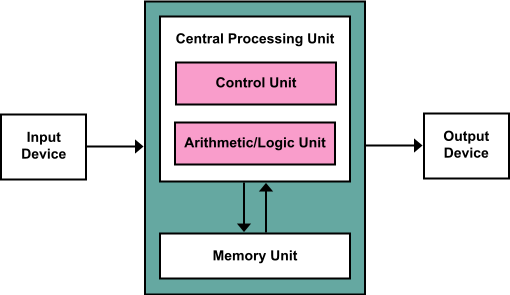
\includegraphics[width=0.6\textwidth]{Von_Neumann_Architecture.png}
\caption{Von Neumann Architecture~\cite{vonNeumanngfx}}
\label{fig:vonNeumanng}
\end{figure}

We can apply the definition of Von Neumann's Architecutre to further categorize two IoT edge devices:
\begin{itemize}
\item A \textbf{Micro controller unit (MCU)} is an integrated, fully capable, self sufficient computer on a sincle chip. It can run a "bare metal interface", meaning that it doesn't require to run an OS. Without which, it can run a single thread, or a controll loop, forever. As the title of this thesis implies, MCUs are the main focus of this thesis. 
\item A \textbf{Micro processor unit (MPU)} requires support from surrounding chips that enable various functionalities like memory, interfaces, and I/O and cannot act as a stand alone computer. The MPU, according to the Von Neumann's Architecture, is just the processor unit.
\end{itemize}
While the above terms, MCU and MPU, are oftentimes used interchangably, we want to point out the differences of these two families. It is far easier to run an OS such as the Linux Kernel \cite{raspberrypios} on MPU enabled devices, such as the Raspberry Pi 4, because it is not limited to the capabilites on the chip, and can easily be extended with, i.e. more RAM~\cite{raspberrypi4}. A MCU is limited to the design and capabilities of the chip. Hence, a MPU runs with far higher processing capability and much larger applications, while MCUs are for lightweight computing where the OS, if one decides to use one, is integrated on-chip. 
But because some MCUs have straightforward software drivers for more complex peripherals and more MPUs are available that have integrated peripherals on-chip, the gap between MCUs and MPUs is becoming less evident~\cite{peterson2021mcu, thornton2017mcu}.
%

\section {Processors}
When compiling software for a target platform, one must be aware of the different instruction set architectures (ISA) of the target CPUs. Listed below are the most noteworthy processor families that we came across.

\begin{itemize}
\item \textbf{ARM Cortex-M-Series}, are 32-bit RISC processors, designed for low-cost, low-power, and usually embedded in MCUs and other IoT devices~\cite{cortexm}.
\item \textbf{ARM Cortex-A-Series}, are 32-bit or 64-bit RISC processors, in contrast to the Cortex-M-Series, these processors have higher energy consumption that are built for more complex tasks such as supporting an OS~\cite{cortexa}.
\item \textbf{Tensilica Xtensa}
\end{itemize}

As description of the ARM Cortex-M processors seems to fit our premise perfectly, the low-cost and MCU aspect, we will focus on these types of CPUs


\section{Market Analysis}

[MAYBE MOVE THIS CHAMPTER TO THE IMPLEMENTATION?]

To find a suitable MCU that could support Linux, a market analysis had to be performed. The most relevant criteria where having sizable RAM preferably more than 1MB, more than 40MHz CPU clock rate, availability in the region, and a large community because this can simplify development due to the availability of online ressources. Furthermore with the homogenious nature of IoT, directing this thesis towards a smaller target audience would inevitably decrease its value.

\begin{sidewaystable}[]
	\centering
	\begin{tabular}{c|c|c|c|c|c|c|c|c}

	\textbf{Manufacturer} 	& \textbf{Chip/Dev Board} & \textbf{Classification} & \textbf{CPU} & \textbf{ISA} & \textbf{bit} & \textbf{Clock rate} & \textbf{RAM} & \textbf{Flash} \\
	\hline
	\hline
	Raspberry Pi          	& Raspberry Pi 4   	& MPU  	& ARM          & Cortex-A72   	& 64    	& 1.5GHz		& 2-8GB (SDRAM)		& asdf\\
	Raspberry Pi          	& Zero 2 W          	& MPU   	& ARM          & Cortex-A53   	& 64     	& 1GHz		& 512MB (SDRAM)		& asdf\\
	Raspberry Pi          	& Pico           		& MCU   	& ARM          & Cortex-M0+   	& 32 	& 133 MHz 	& 264kB (SRAM)	 	& 2MB\\
	\hline
	Espressif             		& ESP32               & MCU   	& Tensilica    	& Xtensa       		& 32		& 240 MHz	& 520kB (SRAM)		& adsf\\
	Espressif             		& ESP32-S2    	& MCU   	& Tensilica    	& Xtensa       		& 32		& 240 MHz	& 320kB (SRAM)		& asdf\\
	Espressif             		& ESP32-C3    	& MCU   	& RISC-V       & RISC-V       	& 32		& 160 MHz	& 400kB (SRAM)		& asdf\\
	Espressif             		& ESP32-S3     	& MCU   	& Tensilica    	& Xtensa       		& 32		& 240 MHz	& 512kB (SRAM)		& asdf\\
	\hline
	STMicroelectronics  	& STM32F0     	& MCU   	& ARM          & Cortex-M0    	& 32		& 48MHz		& 4-32kB				& asdf\\
	STMicroelectronics  	& STM32F1     	& MCU 	& ARM          & Cortex-M3    	& 32		& 72MHz		& 4-94kB				& adsf\\
	STMicroelectronics  	& STM32F3       	& MCU  	& ARM          & Cortex-M4    	& 32		& 72MHz		& 16-80kB (SRAM)		& asdf\\
	STMicroelectronics  	& STM32F4       	& MCU  	& ARM          & Cortex-M4    	& 32		& 180MHz	& 256kB (SRAM)		& asdf\\ % correct this
	STMicroelectronics  	& STM32G0        	& MCU  	& ARM          & Cortex-M0+   	& 32		& 64MHz		& 144KB (SRAM)		& asdf\\
	STMicroelectronics  	& STM32L4       	& MCU   	& ARM          & Cortex-M4    	& 32		& adsf		& adf 				& adf\\ % correct this
	STMicroelectronics  	& STM32G4       	& MCU   	& ARM          & Cortex-M4    	& 32		& 170 MHz	& 128-512KB (CCM-SRAM)& asdf\\ % correct this
	\hline
	Arduino               		& Due A000062    	& MCU  	& ARM          & Cortex-M3    	& 32       & 84MHz		& 96KB (SRAM)		& asdf \\         
	\end{tabular}
	\caption{Market analysis of available IoT edge devices}
	\label{tab:market}
\end{sidewaystable}

With the insights of the market analysis, see table \ref{tab:market}, and the realization that the required MCU on-chip RAM might not suffice for running Linux, a multitude of sales representatives of hardware manufactureres primarily of STM, were contacted. Among others, Digi-Key Electronics, Anatec AG, Avnet Silica Rothrist and Mouser Electronics. Questions concerning extensibility of RAM were posed with the goal of gaining expert insight. For the purposes of this thesis, more RAM was required.

[MENTIONE: I arranged the boards from STM to get some support.]

\begin{figure}
\centering
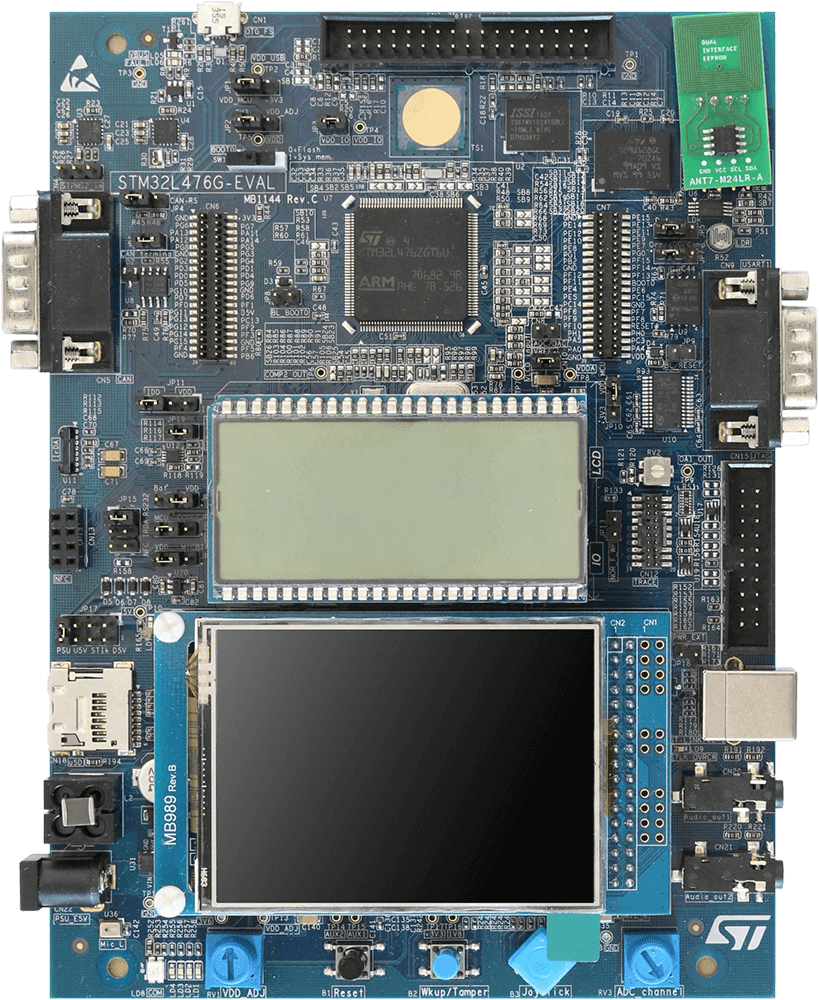
\includegraphics[width=0.6\textwidth]{stm32l476g-eval.png}
\caption{STM32L476G-Eval development board~\cite{stm32Lpic}}
\label{fig:stm32l}
\end{figure}
THE PICTURE ------>\cite{stm32Lpic} \figref{stm32l}

[ADD PICTURE OF THE ESP32 WROOWIE]

\section{Toolchains, Cross-Compilation \& Libraries}\label{toolchains}
For compiled languages, the appropriately name toolchain combines multiple steps into a single pipeline, to produce binary, or machine code. Each step in the process is a piece of software that fullfils its role or function, and hands work over to the next tool in the chain. Interpreted languages such as Python do not require compilation or toolchains, the interpreter executes, or interprets, the code directly. Since this thesis focuses on code than runs closely to hardware, interpreted languages are not concidered. When compiling code a multitude of factors need to be concidered when choosing a toolchain, because they are specifically designed to work excusivley in the right circumstances. Most importantly, whether the host platform is the same as the target platform. The host is the platfrom on which the compilation takes place, and the target on which the binaries will evenually end up running on. If host and target platfrom are not the same, then we speak of cross-compilation. Another important aspect of cross-compilation is the fact that, especially in our case, the target platform may lack computing power and memory, thus compiling could be very time inefficient or simply be impossible. If compilation in mentioned, cross-compilation is implied, since the goal of this thesis is not to evaluate binary code compiled for the host system, but for the target system, being the MCU edge devices. Broadly simplified toolchains work as follows.

As mentioned, the first tep in a toolchain is source code compilation. Depending on the programming language the source code was writen in, compiler vary. For different compiled languages such as C and C++ different compilers are required. In our case, C is of primary concern because the linux kernel is mostly (98.4\%) written in C~\cite{githubLinux}. From each source file that was compiled in the first step result Assembly code. Assembly code, marked with ending \code{.s}, is a set of simplified instructions and basic operations, in other words its a human readable abstraction of maschine code, i.e. bits.
Nowdays Assembler programming is only utilized in situations when extremely efficient management of processor activities is required, but it is still an intermediate-product in compilation. Assebly code needs to be assembled outputing object code. Finaly the object code files need to be linked with required libraries to form an, either statically or dynamically linked, executable, see section \ref{dsll}. After successful cross-compilation follows only execution on target device, which might seem like the easiest step, this is further discussed in section \ref{flashing.ch}.

For the goals of this tesis, we will be compiling, mostly, C code on host platform operating on \code{x64} architecture for target platforms on \code{Armv7E-M} architecutre. Hence cross-compilation will take place with the \code{gcc-arm-none-eabi} toolchain~\cite{gcc-arm-none-eabi}.

[INCLUDE GRAPHIC FOR COMPILATION]

\subsection{Dynamically \& Statically Linked Libraries}\label{dsll}
A Library is a collection of precompiled and reusable components that hold functionality for common processes. The most common example for such a library is C's \code{stdio.h} which hold, among others, function \code{fprintf}, which simply prints characters to the console. As previously stated there are two main methods of linking such functions with the executables, we distinguish between statically linked libraries (SLL) or static libraries, and dynamically linked libraries (DLL) or shared libraries. SLL is the simplest form, as when linking, the contents of the library, specifically the required functions, are included in the executable file. On a small scale this doesn't pose any problems, yet with more exectuables that are loaded into memory, each of these executables contain their own SLL. This can lead to the RAM (or ROM) being occupied by the same function multiple times. Especially when RAM is limited, as is in our case, the redundancy of the same function is not desired. DLL on the other hand requires only one instance of the functionality, all the executables that require this specific function, can access the read-only segment of the library, therefore it can be shared. This process of sharing libraries is aided by a hardware solution, the MMU, see section~\ref{mmu.ch}.

Once again, for our purposes dynamically linked executables are required, since we want to save as much space as possible, thus only linking the required functions and not the entire library. 
%

\subsection{Buildroot }\label{buildroot.ch}
Buildroot is a tool that makes cross-compiling a complete Linux system for an embedded devices easier and more automated. It runs primarily on Linux systems. Through the use of this facilitated toolchain, it creates a self compressing version of the Linux kernel \code{zImage}, a root filesystem, a U-boot bootloader, and root file system and an SD card image file \code{sdcard.img}~\cite {buildroot}.

\subsection{Yocto Project \& OpenWrt}
Equivalently to Buildroot, the Yocto Project and OpenWrt are tools used for Linux cross-compilation for embedded systems. OpenWrt has a focus on Netoworking, the Yocto Project does not currently support MMU-less builds.~\cite{openwrt, yocto}. These tools are not used in this thesis but fill a similar role as Buildroot and are mentioned for the sake of thoroughness. 

\section{Memory Management Unit}\label{mmu.ch}
The Memory Management Unit (MMU) is hardware that is positioned between the processor and physical memory. If present, memory references from the software, through the processor, are passed through the MMU, which in turn maps these references to the actual memory, where the data being called actually resides. In more techtical terms, the reference points to a virtual memory addresses that the MMU can translated into the physical memory addresses. Hence, the program running on the CPU can doesn't need to know the physical memory address. This can simplify addressing in complicated systems. Furthermore, the MMU facilitates DLL implementation. Linux's memory management system is very complicated and has grown over time, offering a growing number of features, such as \code{nommu} which means MMU-less devices, often MCUs~\cite{linuxMMU1, linuxMMU2}. While the implementation of DLL, for devices that don't contain a MMU device appears to be possible, it once again is very complicated~\cite{sharedLibnoMMU}. There exits Linux variations that are tailored for MMU-less devices, see section~\ref{uclinux}

\section{The Linux Kernel}
The Linux Kernel (Linux) was initially created, by Linus Torwalds, in 1991 for i368 based PCs. After its initial appearance it quickly gained traction among developers, and was licenced under GNU General Public License (GPL) as free OSS~\cite{linuxlicense}. At current time, Linux supports all kinds of different target architectures, and dominates that IoT market~\cite{sabri2017comparison}.


\subsection{$\mu$Clinux}\label{uclinux}
The open source nature of Linux made it possible to fork the source code and modify it according to ones needs. One such project is the $\mu$Clinux, which was specifically created to target MMU-les microcontrollers. Its hardware dependent, such as physical memory, and independent code, such as virtual memory, are distinct. Using the given instructions, the hardware-specific portion may be altered for a number of CPUs, hence the OS is modifiable. The system supports both user-space and kernel-space, and switching between the two may be done using system calls. It is possible to develop in a multi-threading environment using POSIX thread libraries. Neither a virtual memory model nor an memory protection unit exist, but functions can be used to dynamically allocate memory, hence DLL is possible. It features a complete TCP/IP stack that may be swapped out for a lighter stack like uIP or lwIP~\cite{dunkels2003full}. But, in comparison to other IoT edge device OSs, as seen in section \ref{iotos}, $\mu$Clinux has a far larger footprint than other IoT OSes~\cite{gaur2015operating}. $\mu$Clinux was eventually discontinued as a standalone fork and was reintroduced into the mainline Linux kernel. With the official emailing list gone quiet and its webpage only visible through web archives, and the last official update publish in May of 2016~\cite{uclinux.org}. Other entities appear to have forked and maintained it further down the line, such as emcraft~\cite{emcraft, emuClinux}, with last comits on December 2017, one year later. The last remaining verifiable remnants appear to be pointing towards a "small C library for developing embedded Linux systems" called uclibc-ng~\cite{uclibc-ng}, which could prove useful.

\section{U-Boot}
"Das U-Boot" is an open source boot loader used predominantly in embedded devices. It's main focus is to load the OS kernel into main memory. It supports a wide variety of IoT development boards~\cite{u-boot-doc}. Yet again, as is common in the IoT ecosystem, there is a multitude of U-Boot forks, the original and the one that appears to be maintained and updated most frequently is by denx, while the previously mentioned emcraft has their own~\cite{emUboot}. 

When not otherwise mentioned, when U-Boot is mentioned we are refering to U-Boot maintained by denx~\cite{u-boot}.

\section {QEMU}\label{qemu.ch}
Primarily a general-purpose machine virtualizer and emulator, QEMU has a variety of applications. In this thesis we will use it to emulate a system, thus creating a virtual replica of a MCU, including the CPU, memory, and simulated peripherals, in order to run a compiled version of Linux. The CPU may operate in this mode entirely emulated or in conjunction with a hypervisor like KVM, Xen, Hax, or Hypervisor. Equivalently to the cross-compilation process that was dicussed in section \ref{toolchains}, the "user mode emulation," allows QEMU to run programs that were built for the target CPU, on our host CPU~\cite{qemu}.


\chapter{Standarizing the IoT OSs with Linux}

In this chapter, we propose a way toward standardizing the heterogeneous IoT edge device ecosystem with Linux. While not an easy task and with many stepping stones on the way, there certainly are a multitude of benefits that such a consensus would bring.

\section{Proposal}\label{proposal.ch}
As the layer between the user and the hardware, an OS provides an interface with which the former can input data, perform calculations and view the output. OSs can be seen as a standardized layer. An interface can be implemented such as a graphical user interface (GUI), or a Command Line Interface (CLI). With GUI's having much higher memory requirements, a CLI should provide a lightweight fit for the IoT edge device ecosystem. When it comes to OS choice in IoT, the traditional approach is to choose an real-time operating system (RTOS). While these OSs introduced in Section \ref{iotos.ch}, are technically categorized as operating systems, they should rather be seen as frameworks when compared to Linux. Bare metal code can be written within these frameworks which in turn handles low-level implementations, such as threads and message passing~\cite{jaycarlson}. With increasing computing capabilities, MCUs have surpassed the capabilities of the first PCs running the first operating systems such as UNIX and Linux. To aid the standardization process of IoT this thesis proposes the use of the Linux kernel as a primary OS on edge devices. With projects such as uClinux and Buildroot, with their support for MMU-less devices, this appears beneficial and feasible.

\begin{figure}[H]
\centering
\includegraphics[width=0.8\textwidth]{ba-arch.png}
\caption{Proposed architecture of MCU IoT devices}
\label{fig:ba-arch}
\end{figure}

Illustrated in Figure \ref{fig:ba-arch}, the userspace and the underlying device drivers and hardware are clearly separated from one another. With this level of abstraction, a similar level of user-friendliness, portability, and versatility can be achieved as in laptops and desktops. Precedence for this is the RPI, which has gained widespread use in the IoT industry, partially due to easily supporting Linux.

\section{The benefits and drawbacks of Linux on MCUs}
\textbf{Benefits}

Linux facilitates memory management, protection, and dynamic memory allocation, in section \ref{uclinux.ch} we established that this is possible without an MMU. RTOSs rely on static memory allocation, which can quickly become a problem as applications grow. Problems such as memory leaks and memory fragmentation can force the system to restart, diminishing its real-time aspect. Linux also provides a network stack that removes the requirement to program network applications, and thus ensures interoperability. Furthermore, Linux uses a standardized filesystem, that can be used to reliably manage and store data. Broader language support is another benefit, enabling the use of the same programming languages and libraries across all devices. Applications become much more portable and provide the community with much flexibility. Very interesting use cases arise such as the use of container technology, increasing portability even further. With a large open source community at its back, that maintains and updates the source regularly for many architectures, the adoption of MCU IoT devices into the arenal of Linux, should happen sooner rather than later~\cite{jaycarlson}.

\textbf{Drawbacks}

One might argue that for a slightly higher price, development boards powered by a Cortex-A MPUs, such as the RPI family, are available. These boards could fill the same purpose and have higher computing power, with more RAM and ROM, at the cost of energy efficiency, size, and price. When operating Linux on such small memory, compared to the capabilities of RPI for example, the OS takes up a large proportion of the memory, thus limiting the available space for the applications that need to run on the MCU. Another aspect that needs to be overcome is the larger upfront investment when porting Linux to specific IoT devices, yet with projects such as Buildroot, this is well on the way, if not present already.




\chapter{Implementation}

In this section the general approach is described, aswell as trial and error. One must keep in mind that steps have been boiled down to the most notable. Also all the different tools that were used where expanded as time passed, certainly not all packages and software are required for all steps but where helpfull in building, compiling, flashing and auxillary tasks. 

\section{Work Environment}\label{envsetup.ch}
To provide a portable environment where source code, different tools and toolchains can be placed, a docker container was created. The main advantages of Docker are that tools such as Buildroot \ref{buildroot.ch}, qemu, toolchains, etc are available on Linux. With the additional benefit of the possibilty to automate large parts of the compilation processes through shell scripts, and potentially out sourcing expensiv compilation, in the absence of capable local hardware, to the cloud, Docker seems to be a good fit.

To build a Docker container from an image the Dockerfile is specified in [...........]. The official Ubuntu 20.04 long time support (LTS) baseimage is used. This provides a solid OS with many tools that facilitate aquiering packages with the included packet manager \code{apt-get}. 

A lot of different To install debendencies the installscript.sh is run automatically when building the image. This script includes a variety of different packages that will be required. A set of basic tools enables working inside the container on a CLI, a collection of the most common and broadly used untilies are shown in listing \ref{basic-util}. We use \code{git} and \code{wget} to aquire repositories and files from the internet, a CLI text editor for \code{.config} files, and compressing and uncompressing utility. Any scripts that are displayed, unless specifically stated otherwise, work with the \code{bash} shell.

\begin{lstlisting}[style=SH, caption=Installing basic utility, label=basic-util, float, floatplacement=H]
apt-get install -y git \
wget \
bc \
nano \
curl \
cpio \
unzip \
rsync
\end{lstlisting}

To be able to cross-compile source code to architectures specific binaries for the target device we require further packages, all of which are available on Ubuntu's package manager \code{apt-get}.

\begin{lstlisting}[style=SH, caption=Installing toolchains and dependencies, label=toolchain-util, float, floatplacement=H]
apt-get install -y gcc \
binutils-arm-none-eabi \
make \
gcc-arm-none-eabi \
gcc-arm-linux-gnueabihf \
gcc-arm-linux-gnueabi \
libncurses-dev \
libncurses5-dev \
flex \
bison \
openssl \
libssl-dev \
dkms \
perl \
libelf-dev \
libudev-dev \
libpci-dev \
libiberty-dev \
autoconf \
lzop 
\end{lstlisting}

\section{Sample Code}

To establish a baseline with less complex code compared to the massive source code repepository of the Linux kernel, and all its forks, that can fully be understood, a collection of sample code was found~\cite{sample-code}. These three code snippets, in combination with QEMU as an emulator for target platform, will provide a controlled environment, in which it is easier to verify if compilation was successful and correct, if the binaries works on target platform, or if it was correctly linked. By having such a fall back option it saves  time and power, and provides a solid foundation of the complex processes that occur during cross-compilation. 

\code{notmain.c}, as seen in listing \ref{lst:notmain.c}, writen in the C programming language represents the kernel, which contains the basic loop, with the task of printing the numbers 0 to 7 onto some universal asynchronous receiver-transmitter (UART). Theoretically, if the UART is connected to some console, the output would look something like this:

\code{01234567}

\begin{lstlisting}[style=CEE, caption={notmain.c}\label{lst:notmain.c}, float, floatplacement=H]
void PUT32 ( unsigned int, unsigned int );
#define UART0BASE 0x4000C000
int notmain ( void )
{
    unsigned int rx;
    for(rx=0;rx<8;rx++)
    {
        PUT32(UART0BASE+0x00,0x30+(rx&7));
    }
    return(0);
}
\end{lstlisting}

\begin{lstlisting}[style=ASS, caption={flash.s}, float, floatplacement=H]
.thumb
.thumb_func
.global _start
_start:
stacktop: .word 0x20001000
.word reset
.word hang

.thumb_func
reset:
    bl notmain
    b hang

.thumb_func
hang:   b .

.thumb_func
.globl PUT32
PUT32:
    str r1,[r0]
    bx lr
\end{lstlisting}

\begin{lstlisting}[style=LD, caption={flash.ld}, float, floatplacement=H]
ENTRY(_start)

MEMORY
{
    rom : ORIGIN = 0x00000000, LENGTH = 0x1000
    ram : ORIGIN = 0x20000000, LENGTH = 0x1000
}

SECTIONS
{
    .text : { *(.text*) } > rom
    .rodata : { *(.rodata*) } > rom
    .bss : { *(.bss*) } > ram
}
\end{lstlisting}

To compile this sample code for target platfrom the commands shown in listing \ref{compSample} are issued through the command line shell \code{bash}. Initially starting with three files \code{flash.s}, \code{notmain.c} and \code{flash.ld}, we are now presented with 5 additional files. \code{flash.o}, \code{notmain.o}, \code{notmain.elf}, \code{notmain.list} and most importantly \code{notmain.bin}, the "sample kernel". From listing \ref{compSample} we can also see the flag \code{-mcpu=cortex-m4}, symbolizing that we are compiling for target platfrom ARM Cortex-M4.

\begin{lstlisting}[style=SH, caption=Compiling sample code with gcc-arm-none-eabi toolchain, label=compSample, float, floatplacement=H]
arm-none-eabi-as --warn --fatal-warnings -mcpu=cortex-m4 flash.s -o flash.o
arm-none-eabi-gcc -Wall -O2 -ffreestanding -mcpu=cortex-m4 -mthumb -c notmain.c -o notmain.o
arm-none-eabi-ld -nostdlib -nostartfiles -T flash.ld flash.o notmain.o -o notmain.elf
arm-none-eabi-objdump -D notmain.elf > notmain.list
arm-none-eabi-objcopy -O binary notmain.elf notmain.bin
\end{lstlisting}

\section{Compilation}

\subsection{U-Boot}
As a first step, we will compile U-Boot for QEMU, so that we can continue evaluating, without needing to flash onto an MCU every time. If not previously done so, we need to clone the U-Boot repository, and navigate inside the freshly cloned folder. Using our previously established toolchain, \code{gcc-arm-none-eabi}, we call the commands, shown in listing \ref{compQEMUuboot}, inside of the current folder. At line 2 of listing \ref{compQEMUuboot}, \code{qemu\_arm\_defconfig}, is mentioned after having declared the toolchain. This config is simply a pre-set configuration file that is provided by U-Boot, for specific usecases. After compilation has completed \code{u-boot.bin} is the output of our compilation.

\begin{lstlisting}[style=SH, caption=Compiling U-Boot for QEMU, label=compQEMUuboot]
make mrproper
make ARCH=arm CROSS_COMPILE=arm-none-eabi- qemu_arm_defconfig
make ARCH=arm CROSS_COMPILE=arm-none-eabi-
\end{lstlisting}

\begin{lstlisting}[style=SH, caption=Compiling U-Boot for QEMU, label=compQEMUuboot]
make stm32f469_disco_sd_defconfig
make
\end{lstlisting}

\subsection{Mainline Linux kernel}

[I did this but its pretty pointless, idk. the explorative nature of this thesis had me running against a lot of walls and IDK how to show that. I mean with buildroot, that was found lateron in the thesis, things work easier, but this work here seems to be for nothing.]

\subsection{$\mu$Clinux}

[I did this but its pretty pointless, idk. the explorative nature of this thesis had me running against a lot of walls and IDK how to show that. I mean with buildroot, that was found lateron in the thesis, things work easier, but this work here seems to be for nothing.]


\subsection{Buildroot}
We need to download and navigate to the buildroot directory. In the documentation of Buildroot, under 2.1. "Mandatory packages", a list of required dependencies for the compilation process are shown, we have installed some of these packages in section \ref{envsetup.ch}, and others come with the Ubuntu 20.04 LTS distribution. We are presented with the build root directory shown in listing \ref{buildrootdir}. \code{configs} holds all the pre-set configuration files that can be used to compile Linux, by navigating to the directory we see all the configs that can be used, and lateron modified. Sadly STM32L476G-Eval is not included, but other configurations for STM are available, such as \code{stm32f429\_disco\_xip\_defconfig} for the STM32F429-Discovery development board. \code{make stm32f429\_disco\_xip\_defconfig} will copy the code from the specified configuration into the \code{.config} file, which is not visible in the thee unless command \code{ls -a} is issued. 

\begin{lstlisting}[caption=Buildroot directory, label=buildrootdir]
buildroot/
|
|-- arch
|-- board
|-- boot
|-- configs
|-- docs
|-- linux
|-- package
|-- support
|-- system
|-- toolchain
|-- utils
\end{lstlisting}

Seen in \ref{fig:buildroot-menuconfig}, by typing \code{make menuconfig} will open a visual menu inside the console that can help us visually navigate through the \code{.config} file that was previously set. Note that for this visual editor the \code{libncurses5-dev} package is required and was installed in section \ref{envsetup.ch}.

\begin{figure}
\centering
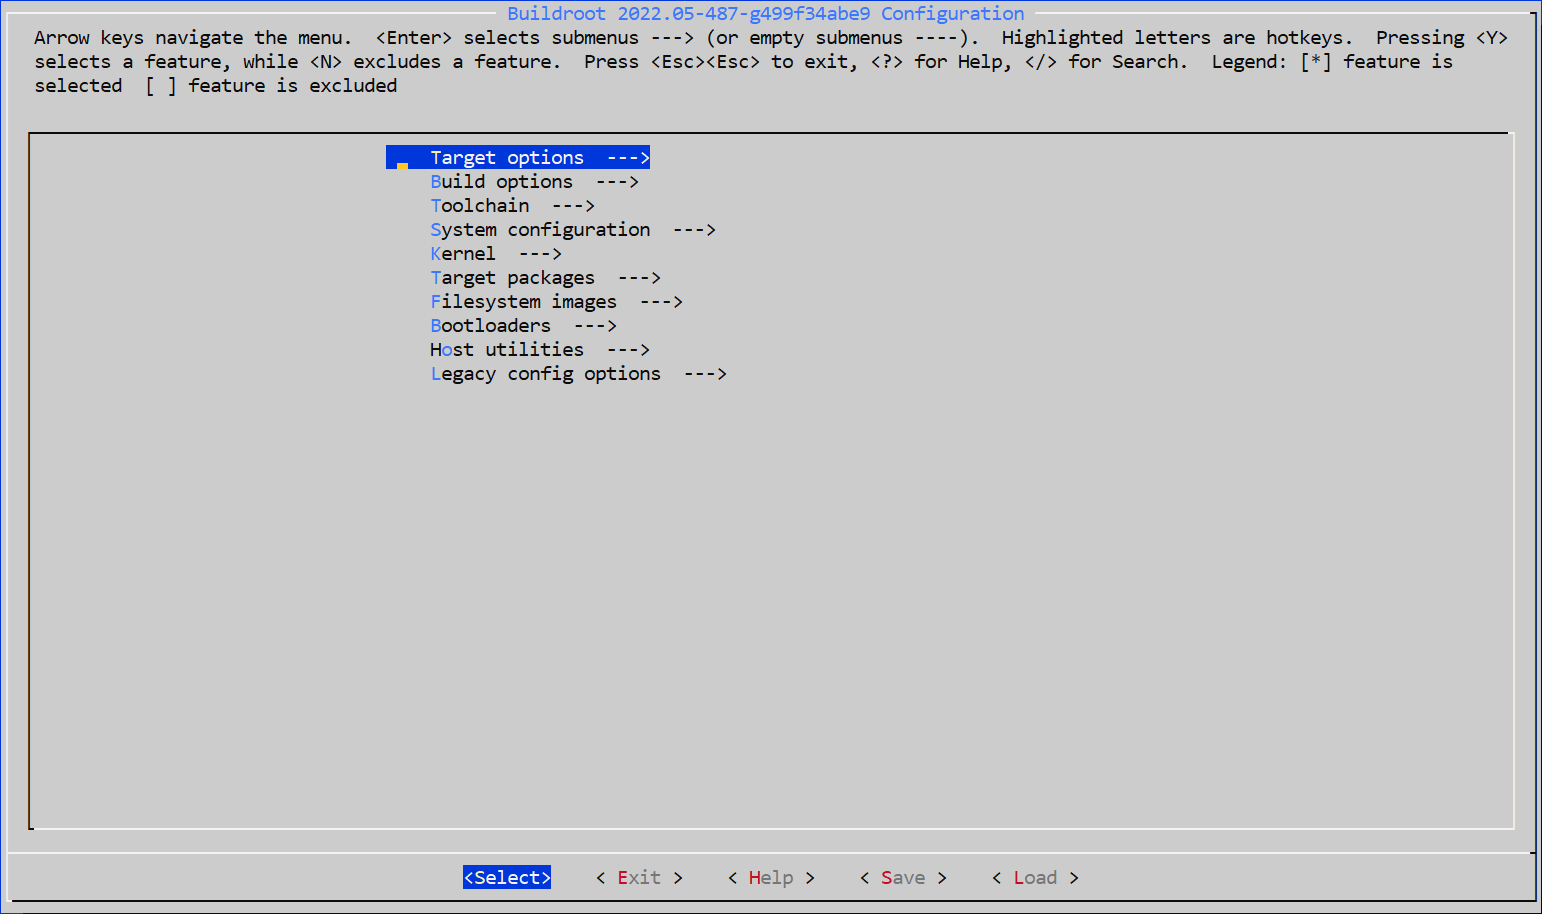
\includegraphics[width=0.6\textwidth]{buildroot-menuconfig.png}
\caption{\code{make menuconfig} inside Buildroot directory}
\label{fig:buildroot-menuconfig}
\end{figure}

With \code{make}, the compilation process starts. Depending on the local maschine that is performing the process, this process can be very time and resource intensive. Once complete, the outputs will appear in a new folder inside the buildroot directory under \code{output}, the contents are shown in listing \ref{buildoutputdir}.

\begin{lstlisting}[caption=Buildroot output directory, label=buildoutputdir]
output/
|
|-- build
|-- host
|-- images
|-- staging
|-- traget
\end{lstlisting}


\begin{lstlisting}[style=SH, caption=Compiling, label=compQEMUuboot]
make stm32f469_disco_sd_defconfig
make
\end{lstlisting}

\section{Proof of Concept}

asdfasdf
\begin{lstlisting}[caption=Installing QEMU in the container]
printf 'y\n8\n7\n' | apt-get install -y qemu-system-arm
\end{lstlisting}
asdfasdf

\begin{lstlisting}[style=SH, caption=Running U-Boot with QEMU, label=compQEMUuboot]
qemu-system-arm -machine virt -nographic -bios u-boot.bin
\end{lstlisting}


\subsection{Setting up $\mu$Clinux}
[maybe irrelevant at this point]

Since the original $\mu$Clinux is not maintained anymore, or rather included in the mainline kernel, and then discontinued. The task of finding an entitiy that has maintained a $\mu$Clinux fork was a daunting task. Emcraft 
Furthermore, scipts that extend this container with additional functionality such as $\mu$Clinux and compatible toolchains~\cite{emuClinux, emUboot}, and Buildroot are provided in init-uClinux.sh and init-Buildroot.sh respectively.

\subsection{Setting up Buildroot}
[maybe irrelevant at this point]


\section{Flashing binaries} \label{flashing.ch}

\section{JuiceVM}
JuiceVM printk() of 1 character for 5 seconds.

\chapter{Evaluation}

[I AM NOT SURE WHAT TO EVALUATE]

\section{QEMU as an evaulation tool}

\section{JuiceVM}

\section{U-Boot}

\section{Mainline Linux kernel}

\section{uClinux}

\section{Buildroot}


\chapter{Summary, Conclusions \& Future Work}

In this thesis, different Linux distributions for IoT edge devices were compiled, with a proposed standardized architecture in the foreground. To achieve this a market analysis of IoT hardware was performed, a variety of tools and open source projects such as Buildroot and JuiceVM were explored and introduced, and Linux and U-Boot binaries were emulated on QEMU. Furthermore, it was attempted to flash Linux binaries onto an STM32L476G-Eval development board which was not successful due to lacking community support for the board, and running a RISC-V emulation on ESP-EYE, which was technically successful but unusable in practice.

The diverse IoT ecosystem and the lack of standardization paired with a manufacturer-driven industry, are the primary justifications for this thesis. The variety of IoT network protocols and OSs, in this these referred to as frameworks rather than OSs, only amplify this heterogeneity. We propose standardization of the OS layer for IoT edge devices, such that an abstraction of the diverse hardware is possible. This would have the effect that board-specific implementations, such as bare metal code, are not required, but that the user can choose from diverse solutions that all work upon the OS layer, therefore the application layer would gain portability.

The process of this thesis was to evaluate possible MCU candidates, that displayed promising qualities, such as sufficient RAM, a CPU with more than 40MHz clock speed while considering energy efficiency and cost. STM in particular showed desired qualities such as a healthy community and the relevant ARM Cortex-M architectures. At this point, contact with STM employees was established and they generously supplied us with two STM32L476G-Eval development boards. Only then did we explore the means to find the right implementation for the desired goal, Linux on MCUs. This thesis concludes that this bottom-up approach is fundamentally flawed, it is not necessarily the hardware that enables the use of Linux, but the community that adapts the kernel to the physical layer. By searching for compatible hardware first, work previously done by the open source community is omitted. The best possible approach to solve a given use case is to compile a list of MCUs that are supported by Linux and tools such as Buildroot, not to choose a board and realize that it is not supported. In such a case, the upfront investment, of porting Linux to a specific board is not worth it. Yet, the explorative nature of this thesis brought forward a different perspective, and different tools such as Buildroot were discovered and evaluated.

Buildroot proved to be an invaluable tool for embedded Linux, as it contains all necessary components such as libraries like the \code{uClibc} and U-Boot. Supporting multiple architectures and subsequently multiple boards, even more so than the mainline Linux kernel. It should further be evaluated with the right boards available. As we performed tests on the STM32L476G-Eval development board, which did not have a dedicated configuration for compilation, we had to adapt configurations of similar boards,  which ultimately did not work because the contrast was too large, as is common in IoT.

While the success of this thesis was evaluated on QEMU in section~\ref{success}, it does not support all the different boards that are available on the market, understandably so. As STM boards were not present but recommendations that similar boards could be emulated instead and that the architecture is similar, yet it did not work as intended. Another aspect that QEMU can not achieve is to verify performance on the target architecture since the underlying hardware is much more capable.

JuiceVM was successfully run, but in practice, it is not a viable or usable solution due to its long boot times. Yet it is a very interesting implementation, and potentially opens up the door to further studies of virtualization on tiny edge devices. Applying such concepts, such as container technology, to tiny IoT devices, if further enhances the portability and versatility of such devices.

Lastly, we provide a modular toolchain container, containing all tools required for embedded Linux, that can be used to cross-compile Linux or $\mu$Clinux kernel, and evaluate their correctness with QEMU.

\bibliographystyle{IEEEtranS}
\bibliography{mybib.bib}


\chapter*{Abbreviations}
\addcontentsline{toc}{chapter}{Abbreviations}
\markboth{ABBREVIATONS}{}

% Introduction
\abr{IoT}{Internet-of-Thingsi}
\abr{RPI}{Raspberry Pi}
\abr{ARM}{Advanced RISC Machines}
\abr{CPU}{Core Processing Unit}
\abr{RAM}{Random Access Memory}
\abr{OS}{Operating System}
\abr{USB}{Universal Serial Bus}
\abr{Wi-Fi}{Wireless-Fidelity}
\abr{RISC}{Reduced Instruction Set Computer}
\abr{CISC}{Complex Instruction Set Computer}
\abr{ISA}{Instruction Set Architecture}
\abr{TEE} {Trusted Execution Environment}
%Realted Work
\abr{RFID}{Network of Radio-Frequency Identification}
\abr{I/O}{Input/Output}
\abr{SoC}{System on a Chip}
\abr{SoM}{System on a Module}
\abr{PCB}{Print-Circuit Board}
\abr{RAM}{Random Access Memory}
\abr{ULP}{Ultra Low Power}
\abr{OSS}{Open Source Software}
% Body 1
\abr{CPU}{Core Processing Unit}
\abr{CU}{Controll Unit}
\abr{ALU}{Arithmetic Logic Unit}
\abr{MCU}{Microcontroller Unit}
\abr{MPU}{Micro-processing Unit}
\abr{DLL}{Dynamically Linked Libraries}
\abr{SLL}{Statically Linked Libraries}
\abr{FMC}{Flexible Memory Controller}
\abr{VM}{Virtual Maschine}
\abr{KVM}{Kernel-based Virtual Machine}
% Body 2
\abr{GUI}{Graphical User Interface}
\abr{CLI}{Command Line Interface}
\abr{RTOS}{Real-Time Operating System}
% Implementation
\abr{UART}{Universal Asynchronous Receiver-Transmitter}
\abr{LTS}{Long Time Support}
\abr{LED}{Light-Emitting Diode}
\abr{GPIO}{General-Purpose I/O}


\chapter*{Glossary}
\addcontentsline{toc}{chapter}{Glossary}
\markboth{GLOSSARY}{}


\begin{description}

  \item[Edge Devices] An edge device refers to perception layer devices, oftentimes powered by an MCU. They are the sensors that reside at the bottom of the chain of IoT, thus called the "edge" device.
  \item[Board] A board refers to a PCB upon which an MCU and peripherals are mounted.

\end{description}



\addcontentsline{toc}{chapter}{List of Figures}
\listoffigures
\addcontentsline{toc}{chapter}{List of Tables}
\listoftables

\appendix

\chapter{Installation Guidelines}

Since a Docker container was used in the thesis, the installation of the toolchains container is very simple. 

\begin{enumerate}
\item Download and install Docker.
\item Download and install Git.
\item Clone the repository provided here \cite{myba}.
\item Inside the directory run command: \code{docker build -t mcu-toolchain:latest .}
\item Then run \code{docker run -it mcu-toolchain:latest}.
\end{enumerate}

You have successfully installed the container, and are currently inside it.

\chapter{Contents of the CD}
\begin{itemize}
\item STM32CubeIDE project containing source code based on FreeRTOS toggling the LED.
\item Docker container
\item Installation files for all utilities used.
\item Thesis with latex files and the graphics.
\item Final presentation
\item JuiceVM folder
\end{itemize}


\end{document}
